\documentclass[tikz]{standalone}
\usepackage{pgfplots}
\pgfplotsset{compat=1.15}
\usepackage{mathrsfs}
\usetikzlibrary{arrows,calc}
\usepackage{tkz-euclide}
\pagestyle{empty}

\definecolor{AngleClr}{rgb}{0,0.39215686274509803,0}
\definecolor{ShapeClr}{rgb}{0.6,0.2,0}
\definecolor{SquareClr}{RGB}{250, 248, 217}


\begin{document}

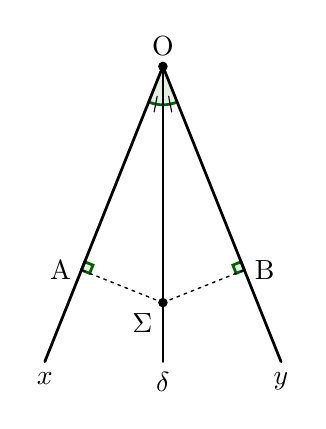
\begin{tikzpicture}[scale=.75]
\tkzSetUpLine[line width=1pt,color=black]
\tkzSetUpPoint[fill=black]

\tkzDefPoints{0/0/x,2/5/O,4/0/y,2/0/d,2/1/S}


\tkzDefPointBy[projection=onto O--x](S)\tkzGetPoint{A}
\tkzDefPointBy[projection=onto O--y](S)\tkzGetPoint{B}

\tkzMarkRightAngle[line width=1pt, size=.15,color=AngleClr,fill=AngleClr,fill opacity=0.1](S,A,O)
\tkzMarkRightAngle[line width=1pt, size=.15,color=AngleClr,fill=AngleClr,fill opacity=0.1](S,B,O)


\tkzFillAngle[fill=AngleClr,size=.65,fill opacity=0.1](A,O,S)
\tkzMarkAngle[line width=1pt,size=.65,color=AngleClr,mark=|,mksize=3](A,O,S)

\tkzFillAngle[fill=AngleClr,size=.65,fill opacity=0.1](S,O,B)
\tkzMarkAngle[line width=1pt,size=.65,color=AngleClr,mark=|,mksize=3](S,O,B)

\tkzDrawSegment[line width=0.5pt,color=black,dashed,dash pattern=on 1pt off 1.75pt](S,A)
\tkzDrawSegment[line width=0.5pt,color=black,dashed,dash pattern=on 1pt off 1.75pt](S,B)
\tkzDrawSegment[line width=1pt,color=black](x,O)
\tkzDrawSegment[line width=1pt,color=black](y,O)
\tkzDrawSegment[line width=1pt,color=black](d,O)


\tkzDrawPoints[size=3](S,O)



\tkzLabelPoint[below](x){$x$}
\tkzLabelPoint[below](y){$y$}
\tkzLabelPoint[below](d){$\delta$}
\tkzLabelPoint[below left](S){$\mathrm{\Sigma}$}
\tkzLabelPoint[left](A){$\mathrm{A}$}
\tkzLabelPoint[right](B){$\mathrm{B}$}
\tkzLabelPoint[above](O){$\mathrm{O}$}

\end{tikzpicture}

\end{document}
